%al posto di template.tex va messo il nome del file del livello superiore
\documentclass[../RiunioneInterna16-02-19.tex]{subfiles}

\begin{document}
\section{Verbale della riunione}
Di seguito sono elencate le decisioni prese durante la riunione odierna:
\begin{itemize}
\item \textbf{Documenti:}
	\begin{itemize}
		\item PP: il preventivo è stato rifatto, come il consuntivo PP, e il resoconto PQ;
		\item PQ: è necessario aggiungere la possibilità di esportare il resoconto e i test da Tracy;
		\item NP: è necessario rivedere alcune norme e aggiungere agli strumenti jenkins;
		\item AR: è stato deciso di aggiungere un nuovo use-case e di spezzare quelli non atomici come prossima attività.
	\end{itemize}		
		
\item \textbf{Strumenti:} è stato deciso che l'hook post-commit del repository sarà gestito su sistemi Linux e adattato successivamente per sistemi Windows;


\item \textbf{Specifica tecnica:}
	È necessario risolvere l'accesso al database SQLite, si propone di utilizzare un framework tra Sugar o ORM ma richiedono delle prove per comprendere meglio il da farsi.
	Il componente model manca della parte del database e della rilevazione Beacon. Si è deciso di non fare alcun diagramma di attività.
	
	
\item \textbf{Prototipo:}
	Visti i ritardi e la mole di lavoro ancora da fare non ci sarà nessuna creazione del prototipo.

\item \textbf{Definizione di prodotto:}
	Si è deciso di iniziarla nel momento in cui la progettazione della business logic dell'applicativo è terminata.
	
\item \textbf{Altro:}
	\begin{itemize}
		\item Chiedere al professore ulteriori approfondimenti per la gestione delle interruzioni nei diagrammi delle attività;
		\item Inviare mail a Miriade per confermare l'avvenuta consegna di altri 25 beacon;
		\item Verrà aperta una nota su Teamwork per elencare i quesiti per l'incontro col proponente;
		\item In seguito alla mail di risposta del proponente, che riportiamo evidenziata nella conclusione del presente verbale \ref{mail}, il requisito \textbf{ROpzV3.3.1.4} verrà meglio specificato come sollevato dalla revisione dei requisiti.
	\end{itemize}
	
\end{itemize}

	\begin{figure}
		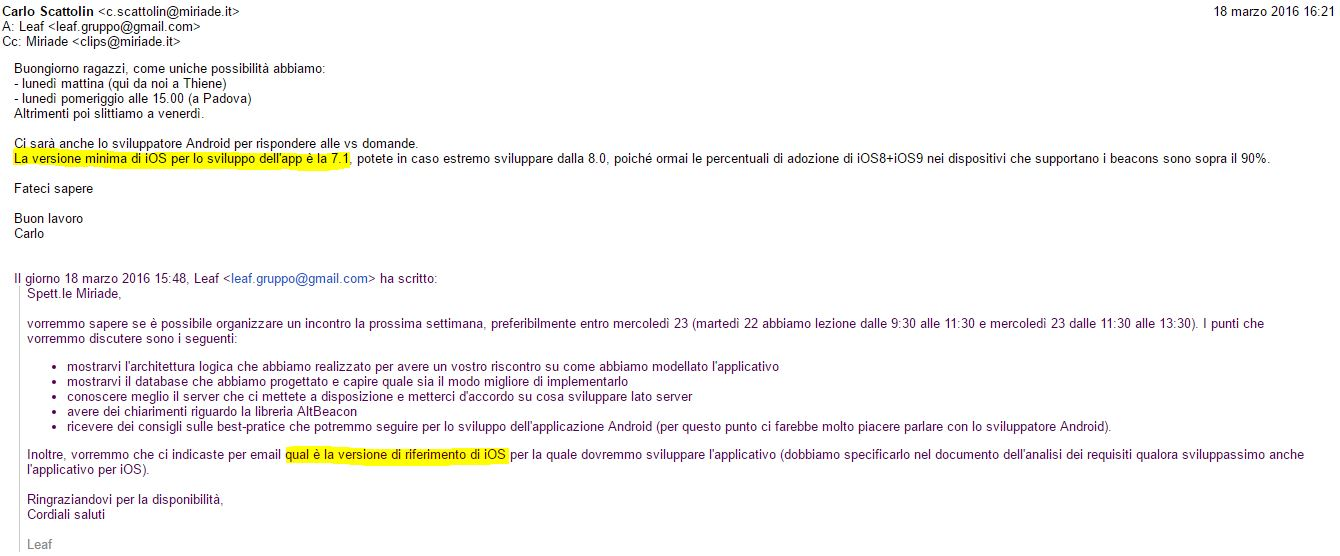
\includegraphics[width=\textwidth]{img/mail}
		\caption{Mail ricevuta il 2016-03-18 dal proponente in risposta alla richiesta della versione di riferimneto per iOS }		
		\label{mail}
	\end{figure}
	\hfill

\end{document}

